\documentclass{article}
% FMTS @ NeurIPS 2026 camera-ready. Body up to 4 pages excluding references and appendices; non-archival.
% Submission version (as reviewed): fmts_submitted.tex. Camera-ready due 6 Nov 2026.
% Figures: paper/scripts/fmts_figures.py (modes, protocols, ts_transfer_sd), experiments/transfer/qsweep.py (qsweep),
% paper/scripts/draw_architecture.py (architecture).
\usepackage[dblblindworkshop,final]{neurips_2026}
\workshoptitle{FMTS}
% Shared packages for NeurIPS 2026 workshop copies. Load neurips_2026 and
% \workshoptitle before inputting this file. Compile from paper/workshops/ with
% TEXINPUTS=..: (see build.sh).
\usepackage[utf8]{inputenc}
\usepackage[T1]{fontenc}
\usepackage{hyperref}
\usepackage{url}
\usepackage{booktabs}
\usepackage{amsfonts,amsmath,amssymb}
\usepackage{microtype}
\usepackage{xcolor}
\usepackage{graphicx}
\usepackage{subcaption}
\usepackage{multirow}
\usepackage{float}
\graphicspath{{../figures/ts/}{figures/ts/}}
\newcommand{\NParamsMain}{5,285}
\newcommand{\MainClAR}{0.046}
\newcommand{\MainCdAR}{0.0036}
\newcommand{\MainStallCd}{0.0060}
\newcommand{\MainClTF}{0.046}
\newcommand{\MainCdTF}{0.0036}
\newcommand{\MainFusedUs}{81}
\newcommand{\MainFusedCachedUs}{58}
\newcommand{\MainEagerMs}{0.89}
\newcommand{\MainMpsUs}{43}
\newcommand{\MainDraftCl}{0.100}
\newcommand{\MainStreamTeightUs}{10}
\newcommand{\TinyParams}{482}
\newcommand{\TinyClAR}{0.100}
\newcommand{\TinyCdAR}{0.0083}
\newcommand{\TinyFusedUs}{38}
\newcommand{\TinyFusedCachedUs}{31}
\newcommand{\PlainClAR}{0.076}
\newcommand{\PlainCdAR}{0.0052}
\newcommand{\OldClAR}{0.137}
\newcommand{\OldCdAR}{0.0107}
\newcommand{\OldClTF}{0.129}
\newcommand{\OldCdTF}{0.0082}
\newcommand{\MidParams}{2,373}
\newcommand{\MidClAR}{0.057}
\newcommand{\MidCdAR}{0.0044}
\newcommand{\MidFusedUs}{61}
\newcommand{\NFxxsCl}{0.092}
\newcommand{\NFxxsCd}{0.0128}
\newcommand{\NFxxsStallCd}{0.0256}
\newcommand{\NFxxsLatMs}{0.57}
\newcommand{\NFxxxlCl}{0.082}
\newcommand{\NFxxxlCd}{0.0115}
\newcommand{\NFxxxlStallCd}{0.0239}
\newcommand{\NFxxxlLatMs}{4.63}
\newcommand{\SeedClMean}{0.048}
\newcommand{\SeedClStd}{0.004}
\newcommand{\SeedCdMean}{0.0037}
\newcommand{\SeedCdStd}{0.0002}
\newcommand{\SeedStallCdMean}{0.0062}
\newcommand{\SeedStallCdStd}{0.0003}
\newcommand{\SeedN}{3}
\newcommand{\MainGpuMJ}{3.2}
\newcommand{\MainGpuPolarsPerS}{53k}
\newcommand{\MidGpuMJ}{2.0}
\newcommand{\MidGpuPolarsPerS}{86k}
\newcommand{\TinyGpuMJ}{1.1}
\newcommand{\TinyGpuPolarsPerS}{160k}
\newcommand{\PlainGpuMJ}{2.8}
\newcommand{\PlainGpuPolarsPerS}{62k}
% ---- physics-lever study (WHISP pool: held-out-geometry val, 63,548 polars / 4.27M points; 4 seeds) ----
\newcommand{\PhysParams}{5,803}
\newcommand{\PhysClAR}{0.0416}
\newcommand{\PhysClStd}{0.0014}
\newcommand{\PhysCdAR}{0.00342}
\newcommand{\PhysCdStd}{0.00010}
\newcommand{\PhysStallCd}{0.0059}
\newcommand{\PhysStallCdStd}{0.0002}
\newcommand{\PhysSeedOneCl}{0.0426}
\newcommand{\PhysSeedOneCd}{0.00349}
% physics-ablation baselines (same WHISP held-out val, 4 seeds each)
\newcommand{\BaseParams}{5,285}
\newcommand{\BaseClAR}{0.0506}
\newcommand{\BaseClStd}{0.0026}
\newcommand{\BaseCdAR}{0.00405}
\newcommand{\BaseCdStd}{0.00011}
\newcommand{\BaseStallCd}{0.00684}
\newcommand{\BaseStallCdStd}{0.00015}
\newcommand{\PhysinvParams}{5,576}
\newcommand{\PhysinvClAR}{0.0462}
\newcommand{\PhysinvClStd}{0.0012}
\newcommand{\PhysinvCdAR}{0.00382}
\newcommand{\PhysinvCdStd}{0.00006}
\newcommand{\PhysinvStallCd}{0.00652}
\newcommand{\PhysinvStallCdStd}{0.00014}
% thirdparty independent-dataset benchmark (pre-WHISP BigFoil pool, 5 seeds, retrained from scratch)
\newcommand{\TpHisCl}{0.0195}
\newcommand{\TpHisClStd}{0.0015}
\newcommand{\TpHisCd}{0.00189}
\newcommand{\TpHisCdStd}{0.00017}
\newcommand{\TpHisSeedOneCl}{0.0271}
\newcommand{\TpHisSeedOneClStd}{0.0013}
\newcommand{\TpHisSeedOneCd}{0.00436}
\newcommand{\TpHisSeedOneCdStd}{0.00200}
\newcommand{\TpPhysCl}{0.0207}
\newcommand{\TpPhysClStd}{0.0023}
\newcommand{\TpPhysCd}{0.00200}
\newcommand{\TpPhysCdStd}{0.00032}
\newcommand{\TpPhysSeedOneCl}{0.0247}
\newcommand{\TpPhysSeedOneClStd}{0.0021}
\newcommand{\TpPhysSeedOneCd}{0.00288}
\newcommand{\TpPhysSeedOneCdStd}{0.00047}
\newcommand{\TpComboCl}{0.0122}
\newcommand{\TpComboClStd}{0.0012}
\newcommand{\TpComboCd}{0.00105}
\newcommand{\TpComboCdStd}{0.00007}
\newcommand{\TpComboSeedOneCl}{0.0137}
\newcommand{\TpComboSeedOneClStd}{0.0022}
\newcommand{\TpComboSeedOneCd}{0.00120}
\newcommand{\TpComboSeedOneCdStd}{0.00008}
% disjoint-pool replication (local BigFoil-family subset, 45.9k polars / 2,500 geometries,
% geometry-disjoint 38,991 train / 6,913 val, retrained from scratch, 3 seeds)
\newcommand{\DisjHisCl}{0.0188}
\newcommand{\DisjHisClStd}{0.0016}
\newcommand{\DisjHisCd}{0.00191}
\newcommand{\DisjHisCdStd}{0.00025}
\newcommand{\DisjHisSeedOneCl}{0.0249}
\newcommand{\DisjHisSeedOneClStd}{0.0022}
\newcommand{\DisjHisSeedOneCd}{0.00350}
\newcommand{\DisjHisSeedOneCdStd}{0.00088}
\newcommand{\DisjComboCl}{0.0114}
\newcommand{\DisjComboClStd}{0.0009}
\newcommand{\DisjComboCd}{0.00098}
\newcommand{\DisjComboCdStd}{0.00003}
\newcommand{\DisjComboSeedOneCl}{0.0127}
\newcommand{\DisjComboSeedOneClStd}{0.0010}
\newcommand{\DisjComboSeedOneCd}{0.00115}
\newcommand{\DisjComboSeedOneCdStd}{0.00003}
% fused-kernel physics overhead (B=1, T=68, median of 2,000 calls, single core)
% M-series (same-run trunk reference 83/60 us); Linux Threadripper for cross-checking
\newcommand{\PhysFusedUs}{99}
\newcommand{\PhysFusedCachedUs}{76}
\newcommand{\PhysFusedLinuxUs}{331}
\newcommand{\PhysFusedLinuxCachedUs}{300}
\newcommand{\BaseFusedLinuxUs}{299}
\newcommand{\BaseFusedLinuxCachedUs}{269}

\IfFileExists{../tables/ts_ko_macros.tex}{\newcommand{\KoBaseCl}{0.047}
\newcommand{\KoBaseCd}{0.0037}
\newcommand{\KoTestBaseCl}{0.047}
\newcommand{\KoTestBaseCd}{0.0037}
}{\newcommand{\KoBaseCl}{--}\newcommand{\KoBaseCd}{--}\newcommand{\KoTestBaseCl}{--}\newcommand{\KoTestBaseCd}{--}}
\setlength{\textfloatsep}{10pt plus 2pt minus 2pt}
\setlength{\floatsep}{8pt plus 2pt minus 2pt}
\setlength{\intextsep}{8pt plus 2pt minus 2pt}
\setlength{\abovecaptionskip}{4pt}
\setlength{\belowcaptionskip}{2pt}
\author{Anonymous authors\\ Paper under double-blind review}

\usepackage{enumitem}
\usepackage{rotating}
\newcommand{\ConsAir}{0.501/0.506}
\newcommand{\ConsEtt}{5.37/5.31}

\author{Avneh Singh Bhatia\\ Exea Labs\\ \texttt{avneh@exealabs.org}}

\title{Streaming for free: one weight vector for the filter and the smoother}

\begin{document}
\maketitle

\begin{abstract}
Many sequence models are used twice: as a \emph{filter} that estimates each step while data arrive, and as a \emph{smoother} that re-estimates every step once the window is complete. In two-stage models a corrector refines a first-pass draft, and a common way to train it, scheduled sampling, lets it read true targets that do not exist at deployment. We train the corrector only on the model's own drafts, and draw a past-only (causal) or full attention mask at random for each batch. On oil temperature, air quality and heart-signal data, every model trained this way has filter and smoother errors within 2\% of each other, and filters within seed spread of a model trained only to filter. Letting the corrector read true targets raises the error of both modes, by up to 25\%. Where future context helps most, a model trained only to smooth smooths 15\% better. With the same recipe, a \NParamsMain-parameter airfoil model streams lift and drag in \MainFusedUs{} microseconds per window on one CPU thread.
\end{abstract}

\section{Introduction}
\label{sec:intro}
Many deployed models read a window of conditions and output one estimate per time step, and they are asked for that output twice. While the window is arriving, the model works as a \emph{filter}: at each step it may use only the inputs seen so far. Once the window is complete, it works as a \emph{smoother}: at every step it may use the whole window, including later inputs (Figure~\ref{fig:modes}a). For example, a model can estimate a power transformer's oil temperature hour by hour from its electrical loads, then re-estimate the same hours at the end of the day with every load known. A small device has room for one set of weights, so the same weights should do both.

We study models with two stages. A \emph{draft} network estimates each step on its own. A \emph{corrector} then reads the drafts of neighbouring steps and outputs the final estimate. Its attention mask is \emph{causal}, meaning each step sees only earlier steps (filter), or \emph{full}, meaning each step sees every step (smoother). A common way to train the corrector is scheduled sampling~\citep{bengio2015scheduled}, which sometimes replaces the drafts it reads with the true targets. We call this \emph{label leakage} (Figure~\ref{fig:modes}b). A leaked target is close to the answer, so the corrector learns to rely on it, and at deployment, where targets are missing, it reads drafts it was not trained on.

\begin{figure}[t]
\centering
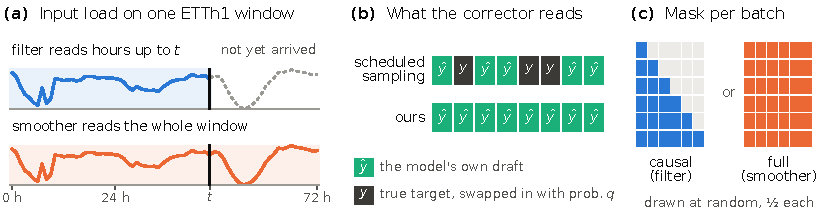
\includegraphics[width=\linewidth]{modes}
\caption{(a) To estimate hour $t$, the filter may read the input (here an ETTh1 load) up to $t$, and the smoother the whole window. (b) Scheduled sampling swaps some of the corrector's inputs for true targets, which do not exist at deployment; our recipe feeds it only drafts. (c) Each training batch uses the causal or the full mask, so one set of weights serves both modes.}
\label{fig:modes}
\end{figure}

Our recipe has two parts. The corrector reads only the model's own drafts, never the true targets, and each training batch uses the causal or the full mask with equal probability. By ``for free'' we mean that adding the filter to a smoother costs no streaming accuracy: the model filters about as well as one trained only to filter. It does not always smooth as well as one trained only to smooth, and we report where it does not. Our contributions are the following.
\begin{itemize}[leftmargin=*,itemsep=1pt,topsep=1pt,parsep=0pt]
\item A comparison of four training protocols on three public tasks (Figure~\ref{fig:protocols}). Models trained under one mask are up to 27\% worse in the other mode. Every model trained with both parts keeps its modes within 2\%, here and on an airfoil task, though in one of six settings a smoothing-only model smooths 15\% better.
\item A sweep over the \emph{leak fraction} $q$, meaning the share of neighbour values replaced by true targets in training (Figure~\ref{fig:sweep}). Leakage raises the error of both modes, by up to 25\%, and costs more when the draft is worse.
\item FoilCORE, a \NParamsMain-parameter airfoil model trained with the recipe, streams in \MainFusedUs\,$\mu$s per window on one CPU thread (Section~\ref{sec:case}); transformer and Mamba correctors trained the same way match it.
\end{itemize}

\paragraph{Related work.} DAgger~\citep{ross2011dagger} and Professor Forcing~\citep{lamb2016professor} address \emph{exposure bias}, the mismatch between training on true previous outputs and running on the model's own, in text generation~\citep{ranzato2016sequence}. Dual-mode speech recognition~\citep{yu2021dualmode,zhang2020u2}, UniLM and UL2~\citep{dong2019unilm,tay2023ul2} already train one network under mixed masks, and our mask draw follows them. Our corrector instead reads a series of its own target, so a leaked label is nearly a copy of the answer.

\section{Training the corrector on its own drafts}
\label{sec:recipe}
We write $x$ for a window's conditions, $y$ for its targets, $\hat y$ for the drafts and $g_\theta(x,\tilde y,m)$ for the corrector, which reads neighbour values $\tilde y$ under mask $m$, causal (c) or full (b, for bidirectional). The \emph{deployment risk} $R_m(\theta)$ is the expected loss when the corrector reads the drafts, as it must in use. Under leak fraction $q$, training replaces each neighbour value by its true target with probability $q$, and we call the expected loss under this scheme the \emph{leaked risk} $\tilde R^q_m(\theta)$. The statements below explain the recipe but do not guarantee that the modes agree (proofs and caveats: Appendix~\ref{app:props}).

\paragraph{Proposition 1 (leakage shifts what the corrector reads).} If the loss changes by at most $L$ per unit change in the corrector's input (in the $\ell_1$ norm), then $|R_m(\theta)-\tilde R^q_m(\theta)|\le L\,q\,\mathbb{E}\|y-\hat y\|_1$. In words, training and deployment losses can differ by an amount that grows with the leak fraction and the draft error. Whenever the draft is imperfect, a leaked target tells the corrector more than the draft does, so training rewards reading it. Setting $q=0$ removes the difference. Because $L$ depends on the weights, the bound predicts a trend, not a size.

\paragraph{Proposition 2 (one objective for both modes).} Drawing the mask with equal probability trains on the average of the two deployment risks, $\tfrac12(R_\mathrm{c}+R_\mathrm{b})$. A \emph{specialist}, meaning a model trained under one mask only, minimizes one term and leaves the other uncontrolled. The average does not ensure that one set of weights reaches both specialists' errors, and Section~\ref{sec:transfer} shows a case where it does not.

\section{Results on three public tasks}
\label{sec:transfer}
We remove every airfoil-specific part and keep a 4k-parameter model: a small pointwise draft network and FoilCORE's two-block attention corrector (Appendix~\ref{app:transfer}). On each task it estimates the target from covariates measured at the same time (\emph{virtual sensing}, not forecasting) and sees no past values of the target. ETTh1~\citep{zhou2021informer} maps electrical loads to oil temperature (96-hour windows), Beijing PM2.5~\citep{liang2015pm25} maps weather to log PM2.5 concentration (72-hour windows), and MIT-BIH~\citep{moody2001mitbih} maps one ECG lead to lead MLII (128 samples, split by patient). We compare draft-only training under the causal mask, the full mask or both (ours) with a label-leaking baseline, three seeds each. The baseline follows \citet{bengio2015scheduled}: $q$ starts at 1 and falls by 0.03 every three epochs, reaching 0 at epoch 103, under the full mask, as our first airfoil model was trained. Every run keeps the checkpoint with the lowest validation error with drafts as input.

\begin{figure}[t]
\centering
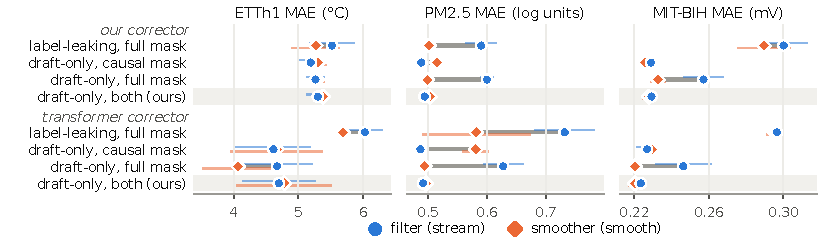
\includegraphics[width=\linewidth]{protocols}
\caption{Test error as a filter (blue, causal mask) and as a smoother (orange, full mask); mean of 3 seeds, whiskers $\pm$1 s.d.\ (values in Table~\ref{tab:transfer}). A long grey bar means the modes disagree. Models trained under one mask are worse in the other mode; draft-only training with both masks (shaded) keeps them within 2\%.}
\label{fig:protocols}
\end{figure}

\subsection{One mask leaves the other mode worse; both masks keep them together}
Specialists are worse in the mode they were not trained for (Figure~\ref{fig:protocols}). Full-mask specialists stream up to 20\% worse than they smooth (27\% with the transformer corrector), and causal specialists smooth up to 5\% worse than they stream (19\%). The dual-mask model keeps its two modes within 2\% with both correctors, and streams within seed spread of the causal specialist.

The label-leaking baseline is the only protocol whose filter is worse than its smoother on all three tasks (by 5\%, 18\% and 4\%). On PM2.5 and ECG the draft-only full-mask model has a gap at least as large, so the mask explains it; on ETTh1 it has none, so leakage hurts the filter. How much leakage adds depends on where the schedule stands when validation error stops improving: on ECG the kept checkpoints come after one or two epochs, when nearly every neighbour value is a target, and the baseline is the worst model in both modes; on PM2.5 they come after $q$ has reached 0 (Appendix~\ref{app:transfer}). Section~\ref{sec:sweep} fixes $q$ to isolate leakage.

On ETTh1 with our corrector even the specialists stay within 2\%, as the learned attention is local, and on ECG the corrector barely improves on the draft. Where future context pays, a specialist smooths better: with the transformer corrector on ETTh1, the full-mask specialist smooths at 4.07\,$^\circ$C against 4.78 for the dual-mask model (seed s.d.\ 0.55 and 0.73), so one set of weights does not reach both specialists' errors.

\paragraph{Forecasting foundation models.} Also given the previous hour's target, the 4k model reaches 0.65\,$^\circ$C on ETTh1 in both modes. Zero-shot Chronos-Bolt~\citep{ansari2024chronos}, TinyTimeMixer-r2~\citep{ekambaram2024ttm} and TimesFM-2.5~\citep{das2024timesfm} (0.8M to 231M parameters), forecasting the same hours from 512 past hours of the target without covariates, reach 0.75 to 0.81; the last value gives 0.80 (Appendix~\ref{app:transfer}). Inputs, not size, set the error, and size does not give a forecaster a smoothing mode.

\section{Leakage raises the error of both modes}
\label{sec:sweep}
\begin{figure}[t]
\centering
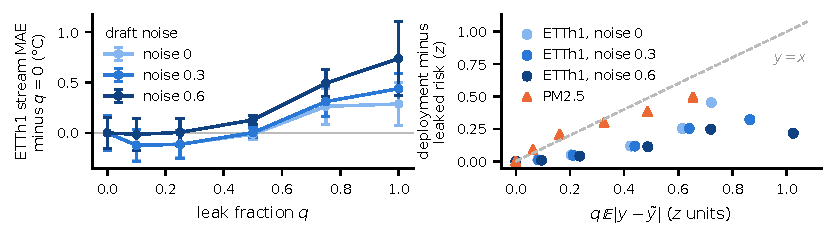
\includegraphics[width=\linewidth]{qsweep}
\caption{Dual-mask training with leak fraction $q$ fixed for the whole run (3 seeds). Left: ETTh1 streaming error relative to $q{=}0$, for three levels of noise added to the draft the corrector reads. Right: deployment minus leaked risk, which Proposition~1 bounds, against the bound's term $q\,\mathbb{E}|y-\tilde y|$. Leaking costs more as $q$ grows, and more with a noisier draft.}
\label{fig:sweep}
\end{figure}

Proposition~1 predicts that the cost of leaking grows with $q$ and with the draft error. We fix $q$ for the whole run under the dual mask (Figure~\ref{fig:sweep}, Table~\ref{tab:sweep}). On PM2.5, streaming error rises steadily from 0.496 at $q{=}0$ to 0.619 at $q{=}1$ (25\%). On ETTh1 it stays within seed spread up to $q{=}0.5$ and reaches 5.59\,$^\circ$C at $q{=}1$ (5.30 at $q{=}0$). To vary the draft error, we add Gaussian noise to the draft the corrector reads. Noise has no effect for $q\le0.25$ and raises the cost for $q\ge0.75$: at $q{=}1$, streaming error is 5.59, 5.75 and 5.95\,$^\circ$C at noise 0, 0.3 and 0.6. The modes stay within 2.3\% of each other at every $q$, so leakage raises the error of both modes, and the gaps in Figure~\ref{fig:protocols} come from training under one mask.

The quantity the bound controls grows with $q$ on both tasks (Figure~\ref{fig:sweep}, right) but not with noise. It depends mostly on how long a run trains on leaked targets (Appendix~\ref{app:transfer}), consistent with the weight dependence of $L$. A consistency-loss baseline that keeps the leaking schedule matches draft-only training once its schedule reaches $q{=}0$, at the cost of two forward passes per batch (Appendix~\ref{app:transfer}).

\section{Case study: a \NParamsMain-parameter airfoil model}
\label{sec:case}
\begin{table}[t]
\centering\scriptsize
\caption{MAE on 34,043 test polars of unseen airfoil shapes, streaming unless marked smooth; parentheses: $C_d$ in stall. NeuralFoil on 1,024 polars. MACs/pt: multiply-accumulates per point. Latency: 68-point polar, one CPU thread.}
\label{tab:main}
\setlength{\tabcolsep}{2.0pt}
\begin{tabular}{lrrrrrrl}
\toprule
Model & Params & $C_l$ & $C_d$ (stall) & smooth.\ $C_l$/$C_d$ & MACs/pt & latency & framework \\
\midrule
FoilCORE-5k (ours) & 5,285 & 0.046 & 0.0036 (0.0060) & 0.046 / 0.0036 & 12.8k & 81\,$\mu$s & C++ kernel \\
FoilCORE-2k ($d{=}16$) & 2,373 & 0.057 & 0.0044 (0.0073) & 0.058 / 0.0043 & 6.1k & 61\,$\mu$s & C++ kernel \\
FoilCORE-3k (plain) & 3,434 & 0.076 & 0.0052 (0.0089) & 0.075 / 0.0052 & 11.8k & 67\,$\mu$s & C++ kernel \\
FoilCORE-0.5k ($d{=}8$) & 482 & 0.100 & 0.0083 (0.0129) & 0.100 / 0.0084 & 2.6k & 38\,$\mu$s & C++ kernel \\
3k, label-leaking & 3,434 & 0.137 & 0.0107 (0.0180) & 0.129 / 0.0082 & 11.8k & 68\,$\mu$s & C++ kernel \\
\midrule
\multicolumn{8}{l}{\emph{Same front-end and protocol, standard backbone as corrector:}} \\
\quad Transformer & 5,822 & 0.048 & 0.0037 (0.0061) & 0.047 / 0.0036 & 8.1k & 166\,$\mu$s & C++ kernel \\
\quad TSMixer & 11,780 & 0.061 & 0.0046 (0.0075) & 0.061 / 0.0045 & 2.4k$^{\ast}$ & 50\,$\mu$s & C++ kernel \\
\quad Mamba (S6) & 5,300 & 0.049 & 0.0038 (0.0063) & 0.049 / 0.0038 & 3.7k$^{\ast}$ & 122\,$\mu$s & C++ kernel \\
\midrule
NeuralFoil xxsmall & 13,302 & 0.092 & 0.0128 (0.0256) & -- & 26k & 0.57\,ms & NumPy \\
NeuralFoil xxxlarge & 1,428,166 & 0.082 & 0.0115 (0.0239) & -- & 2.9M & 4.63\,ms & NumPy \\
\bottomrule
\end{tabular}

\end{table}

We found the problem while predicting airfoil \emph{polars}, the curves of lift and drag coefficients ($C_l$, $C_d$) against angle of attack, which a small drone needs as it pitches. NeuralFoil~\citep{neuralfoil}, a learned model trained on the XFOIL simulator~\citep{xfoil}, does not stream. FoilCORE reads a 200-point airfoil outline and about 75 operating conditions (angle of attack, Reynolds and Mach number) and outputs $C_l$ and $C_d$ for each (Figure~\ref{fig:arch} in Appendix~\ref{app:case}). Labels come from XFOIL (transition setting ncrit\,=\,9) on 5,392 airfoils, split by clusters of near-duplicate shapes so that the 539 test shapes are unseen. As a filter, FoilCORE-5k has a $C_l$ error of \MainClAR{} and a $C_d$ error of \MainCdAR{} (over \SeedN{} seeds, \SeedClMean$\pm$\SeedClStd{} and \SeedCdMean$\pm$\SeedCdStd), and its two modes agree within 1\% (Table~\ref{tab:main}). Transformer and Mamba correctors with the same front end and recipe match FoilCORE, and TSMixer does not; all keep their modes within 2\%. NeuralFoil's largest model is 1.2 to 1.4 times better before stall in incompressible flow at medium Reynolds numbers; FoilCORE is better overall because it takes the Mach number as an input and is 2.7 to 4 times better in stall. A fused C++ kernel runs one polar in \MainFusedUs\,$\mu$s on one CPU thread.

\paragraph{Limitations and when to use the recipe.}
\label{sec:limits}
Airfoil labels come from XFOIL, not measurements, and airfoil ablations are single runs; the public tasks use one small model each and three seeds per cell. In practice: never let the corrector read true targets, draw the mask per batch, and train a full-mask specialist when smoothing accuracy matters most.

\begin{ack}
I thank AMD for compute through the AMD Developer Cloud, accessed through Exea Labs. I trained and evaluated every model in this paper on an AMD Instinct MI300X: the FoilCORE polar predictor and its baselines, the draft--corrector models on ETTh1, Beijing PM2.5 and MIT-BIH (three seeds per protocol), and the zero-shot Chronos-Bolt, TinyTimeMixer and TimesFM-2.5 baselines, up to 231M parameters. Having the foundation-model baselines and the full protocol comparison on one 192\,GB GPU meant every training protocol was run on every dataset, rather than a subset chosen to fit the budget. I thank Daniel Wang at AMD for supporting this work, and the AMD Developer Cloud team for access and help throughout.
\end{ack}

{\footnotesize\setlength{\bibsep}{2pt}
\bibliographystyle{plainnat}
\bibliography{../references}}


\appendix
\section{Public-task details}
\label{app:transfer}
\paragraph{Model (4,234 parameters, $d{=}32$).} Draft: $\mathrm{MLP}(x_t)$ (two GELU layers of width 32, linear head). Corrector tokens: $\mathrm{Linear}([x_t,\tilde y_t])$ plus the draft's hidden state plus a sinusoidal position code; two residual-product-attention blocks (FoilCORE's corrector, \S\ref{app:case}) under a causal or full mask; a linear head adds a residual to the draft. Transformer, Mamba and TSMixer correctors replace the two blocks at widths that keep the model near 4k parameters. The corrector input $\tilde y$ is the detached draft (draft-only) or the label with probability $q$ (leaking).
\paragraph{Data and normalization.} ETTh1: six load channels, hour-of-day and day-of-week (sin/cos), and day-of-year (sin/cos) $\rightarrow$ oil temperature; four-week blocks, every sixth block test and every sixth (offset 3) validation; windows never straddle a block; train stride 8\,h, evaluation stride 24\,h. The lag variant appends $\mathrm{OT}_{t-1}$; with it, the label-leaking twin streams 2.7\% worse than it smooths. PM2.5: dew point, temperature, pressure, cumulative wind speed, snow and rain hours, one-hot wind direction, calendar features $\rightarrow\log(1{+}\mathrm{PM2.5})$; 2010--12 train, 2013 validation, 2014 test. MIT-BIH: 360\,Hz averaged to 90\,Hz, non-overlapping 128-sample windows, records shuffled with seed 0 and split 32/6/10. Inputs and target are $z$-scored with training statistics; MAE is reported in original units.
\paragraph{Training.} Loss: MAE of the final output $+\,0.25\times$ draft MAE. AdamW, learning rate $3\times10^{-4}$, weight decay $10^{-4}$, gradient clipping at 1, learning rate halved after 6 epochs without validation improvement. Batch 64 and at most 150 epochs, patience 25 (ECG: batch 256, 60 epochs, patience 12). Model selection uses validation MAE in the protocol's native mode (causal specialist: causal; bidirectional and leaking: full; dual: the mean), always with the model's own draft as the corrector input. The leaking baseline anneals the draft fraction $1-q$ from 0 by 0.03 every three epochs, so $q$ reaches 0 at epoch 103. Its kept checkpoints (our corrector) come from epochs 1--2 on ECG, 140--149 on PM2.5, and 4, 79 and 88 on ETTh1. Seeds 0, 1, 2. One run takes 20\,s to 2\,min.
\paragraph{Forecasting foundation models.} With $\mathrm{OT}_{t-1}$ appended (one-step-ahead estimation), the dual-mask model reaches 0.652/0.650\,$^\circ$C (stream/smooth). Zero-shot forecasts of the same test hours from 512 past hours of OT: Chronos-Bolt small and base (8.7M, 48M parameters) 0.79 and 0.78, TinyTimeMixer-r2 (0.8M) 0.81, TimesFM-2.5 (231M) 0.75, last value 0.80. A ridge regression on $\mathrm{OT}_{t-1}$ and the covariates reaches 0.65, and 5.8 on the covariates alone (our model: 5.3).
\paragraph{Leak sweep and consistency baseline.} The sweep uses dual-mask training with $q$ fixed for the whole run; draft noise adds $\mathcal N(0,\sigma^2)$ ($z$ units) to the draft the corrector reads, at training and test time, to raise $\mathbb{E}|y-\tilde y|$ without changing the returned draft. The leaked risk is the test MAE with labels substituted at rate $q$. At $q\ge0.75$ on ETTh1, validation error with drafts is often lowest within six epochs. At $q{=}1$ the difference between deployment and leaked risk is 0.15 to 0.25 ($z$) for the six runs kept within six epochs and 0.53 to 0.58 for the three kept after 30 or more; this, not the noise level, sets the spread in Figure~\ref{fig:sweep} (right). The consistency baseline uses the annealed leak, runs both masks on every batch, averages their losses and adds $\|f_\mathrm{c}-f_\mathrm{b}\|_2^2$ (weight 1). Table~\ref{tab:sweep} lists the clean-draft cells. The consistency baseline reaches \ConsEtt\,$^\circ$C on ETTh1 and \ConsAir{} on PM2.5 (stream/smooth), within seed spread of draft-only dual-mask training (5.30/5.38 and 0.494/0.503). Draft-only training gets the same result with one forward pass per batch and no label schedule.

\begin{table}[h]
\centering\footnotesize
\caption{Test MAE of the same 4k-parameter model as a filter (causal mask, ``stream'') and a smoother (full mask, ``smooth''), by training protocol, mean $\pm$ s.d.\ over 3 seeds (the data of Figure~\ref{fig:protocols}). No past target is input. Lower block: a 4.5k-parameter transformer corrector.}
\label{tab:transfer}
\setlength{\tabcolsep}{3pt}
\begin{tabular}{lrrrrrr}
\toprule
Training protocol & \multicolumn{2}{c}{ETTh1 oil temp.\ ($^\circ$C)} & \multicolumn{2}{c}{Beijing PM2.5 (log)} & \multicolumn{2}{c}{MIT-BIH lead II (mV)} \\
 & stream & smooth & stream & smooth & stream & smooth \\
\midrule
label-leaking (sched.\ sampling) & 5.52\,{\scriptsize$\pm$0.35} & 5.27\,{\scriptsize$\pm$0.37} & 0.590\,{\scriptsize$\pm$0.026} & 0.502\,{\scriptsize$\pm$0.004} & 0.300\,{\scriptsize$\pm$0.013} & 0.289\,{\scriptsize$\pm$0.014} \\
draft-only, causal & 5.19\,{\scriptsize$\pm$0.17} & 5.30\,{\scriptsize$\pm$0.13} & 0.489\,{\scriptsize$\pm$0.009} & 0.515\,{\scriptsize$\pm$0.008} & 0.229\,{\scriptsize$\pm$0.001} & 0.226\,{\scriptsize$\pm$0.003} \\
draft-only, bidirectional & 5.26\,{\scriptsize$\pm$0.13} & 5.30\,{\scriptsize$\pm$0.11} & 0.600\,{\scriptsize$\pm$0.012} & 0.499\,{\scriptsize$\pm$0.007} & 0.257\,{\scriptsize$\pm$0.011} & 0.233\,{\scriptsize$\pm$0.004} \\
draft-only, dual mask (ours) & 5.30\,{\scriptsize$\pm$0.17} & 5.38\,{\scriptsize$\pm$0.09} & 0.494\,{\scriptsize$\pm$0.009} & 0.503\,{\scriptsize$\pm$0.005} & 0.229\,{\scriptsize$\pm$0.003} & 0.228\,{\scriptsize$\pm$0.003} \\
\midrule
\multicolumn{7}{l}{\emph{Same, with a transformer corrector in place of ours:}} \\
\quad label-leaking & 6.03\,{\scriptsize$\pm$0.26} & 5.69\,{\scriptsize$\pm$0.04} & 0.732\,{\scriptsize$\pm$0.051} & 0.582\,{\scriptsize$\pm$0.092} & 0.297\,{\scriptsize$\pm$0.004} & 0.295\,{\scriptsize$\pm$0.004} \\
\quad draft-only, causal & 4.62\,{\scriptsize$\pm$0.58} & 4.67\,{\scriptsize$\pm$0.71} & 0.487\,{\scriptsize$\pm$0.007} & 0.581\,{\scriptsize$\pm$0.022} & 0.227\,{\scriptsize$\pm$0.005} & 0.229\,{\scriptsize$\pm$0.001} \\
\quad draft-only, bidirectional & 4.67\,{\scriptsize$\pm$0.54} & 4.07\,{\scriptsize$\pm$0.55} & 0.628\,{\scriptsize$\pm$0.034} & 0.494\,{\scriptsize$\pm$0.003} & 0.246\,{\scriptsize$\pm$0.015} & 0.220\,{\scriptsize$\pm$0.002} \\
\quad draft-only, dual mask & 4.70\,{\scriptsize$\pm$0.56} & 4.78\,{\scriptsize$\pm$0.73} & 0.492\,{\scriptsize$\pm$0.004} & 0.497\,{\scriptsize$\pm$0.003} & 0.223\,{\scriptsize$\pm$0.002} & 0.220\,{\scriptsize$\pm$0.004} \\
\bottomrule
\end{tabular}

\end{table}

\begin{table}[h]
\centering\footnotesize
\caption{Leak-fraction sweep (dual mask, fixed $q$, clean draft; mean of 3 seeds). Negative gap: the stream is more accurate.}
\label{tab:sweep}
\begin{tabular}{lrrrrrr}
\toprule
leak fraction $q$ & 0 & 0.1 & 0.25 & 0.5 & 0.75 & 1 \\
\midrule
ETTh1 stream ($^\circ$C) & 5.30 & 5.18 & 5.19 & 5.29 & 5.57 & 5.59 \\
\quad gap stream$-$smooth (\%) & -1.5 & -1.1 & -0.6 & +0.1 & +0.5 & +1.1 \\
PM2.5 stream (log) & 0.496 & 0.513 & 0.559 & 0.590 & 0.608 & 0.619 \\
\quad gap stream$-$smooth (\%) & -1.6 & -2.3 & -1.9 & -1.4 & -0.7 & -0.6 \\
\midrule
\multicolumn{7}{l}{\emph{Annealed leak + L2 mode-consistency loss:} ETTh1 5.37 / 5.31 (+1.2\%), PM2.5 0.501 / 0.506 (-1.1\%)} \\
\bottomrule
\end{tabular}

\end{table}

\section{FoilCORE details}
\label{app:case}
Width $d{=}32$. Each contour point passes a shared $\mathrm{Linear}(2,d)$ and a per-channel path nonlinearity $\phi$ (Chebyshev series plus a Gaussian bump), pretrained as an autoencoder. Three memories are masked means over the whole contour, the leading edge ($x\le 0.25$) and the trailing edge ($x\ge 0.75$). The fourth is camber and thickness at ten cosine chord stations (a fixed 20-vector) mapped by $\mathrm{Linear}(20,d)$ and $\phi$; dropping it is the largest single loss ($0.047\rightarrow 0.410$ $C_l$). For every $(\alpha,\mathrm{Re},\mathrm{Ma})$ a selective scan~\citep{gu2024mamba,gu2022s4} over the four memories yields a draft $(\hat C_l,\hat C_d)$, and a 16-unit MLP predicts $|\mathrm{draft\ error}|$ (Spearman 0.71 with the $C_d$ residual). Corrector tokens $[\alpha,\mathrm{Re},\mathrm{Ma},\hat C_l,\hat C_d,\hat e]$ plus context and $\mathrm{sinusoid}(\alpha)$ pass two residual-product-attention blocks ($Q{=}K{=}s_1 u+s_3$, $V{=}W_v u$, scores $-\Delta\alpha^2/\tau$, causal or full mask). Loss: MAE on the final output $+\,0.25\times$ draft MAE ($z$-scored, equal weight on $C_l$ and $C_d$) $+\,0.1\times$ error-head L1. AdamW $3\times10^{-4}$, batch 1024, early stopping on causal validation loss (patience 12, at most 300 epochs). Split: 341,135 polars; train 272,748 on 4,313 geometries, test 34,043 on 539; contours resampled to 200 points by arc length. Latency and energy are one thread of an Apple M4 Pro CPU (OpenMP limited to one thread). Energy per polar is at most 0.55\,mJ (idle-subtracted package power from \texttt{powermetrics}, an upper bound). The 3.4k-parameter ``label-leaking'' row of Table~\ref{tab:main} is an earlier model trained with the annealed schedule; it streams 6\% worse than it smooths. Analytic lift and drag priors (518 parameters) lower causal $C_l$ from \BaseClAR{} to \PhysClAR{} on a second data pool over four seeds; they are retrained per pool. Code, weights, split manifest and every number: \url{https://github.com/AvnehSBhatia/FoilCORE}.

\begin{sidewaysfigure}
\centering
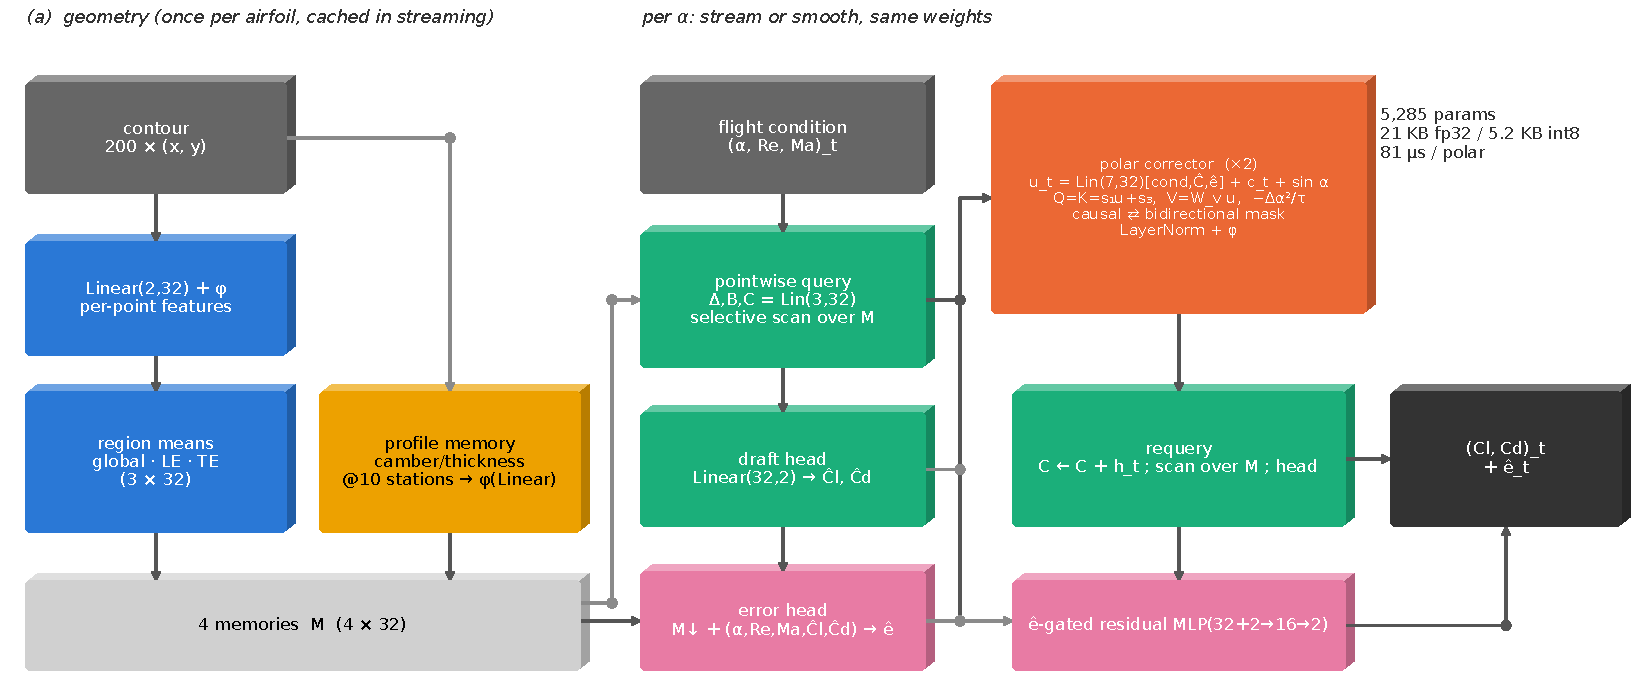
\includegraphics[width=\linewidth]{architecture}
\caption{FoilCORE. A geometry encoder turns the airfoil outline into four summary vectors (memories) once per airfoil; in streaming they are cached. For each angle of attack, Reynolds and Mach number, a selective scan over the memories gives a draft and an error estimate. A two-block attention corrector refines the drafts under a causal or full mask with the same weights.}
\label{fig:arch}
\end{sidewaysfigure}

\section{Propositions: proof and caveats}
\label{app:props}
\paragraph{Proposition 1.} Assume $\tilde y\mapsto\ell(g_\theta(x,\tilde y,m),y)$ is $L$-Lipschitz in $\|\cdot\|_1$. Then $|R_m-\tilde R^q_m|\le\mathbb{E}|\ell(g_\theta(x,\hat y,m),y)-\ell(g_\theta(x,\tilde y,m),y)|\le L\,\mathbb{E}\sum_t|\tilde y_t-\hat y_t|$, and $\tilde y_t-\hat y_t$ equals $y_t-\hat y_t$ with probability $q$ and 0 otherwise, which gives $L\,q\,\mathbb{E}\|y-\hat y\|_1$. The bound does not force the minimizers of the two risks apart: a corrector that ignores the substituted channel is unaffected. $L$ is finite for the correctors we train but depends on the weights.

\paragraph{Proposition 2.} With $m\sim\mathrm{Bernoulli}(\tfrac12)$ the objective is $\bar R=\tfrac12(R_\mathrm{c}+R_\mathrm{b})$, so its minimizer $\bar\theta$ satisfies $R_m(\bar\theta)\le R_\mathrm{c}(\theta)+R_\mathrm{b}(\theta)$ for every $\theta$ and each $m$. This restates what the mask draw optimizes. Reaching both specialists' optima with one weight vector needs the two optima to be compatible, which Section~\ref{sec:transfer} shows is not always the case.

\clearpage
% NeurIPS 2026 paper checklist for the FMTS camera-ready. Does not count toward the page limit.
\section*{NeurIPS Paper Checklist}
\begin{enumerate}\small

\item {\bf Claims.} \answerYes{} The abstract and \S\ref{sec:intro} claim a leakage diagnosis and a training recipe whose dual-mask models stay within 2\% between modes on the public tasks (Figure~\ref{fig:protocols}, Table~\ref{tab:transfer}) and on the airfoil (Table~\ref{tab:main}); the leak-fraction sweep (\S\ref{sec:sweep}) supports the claim that leakage raises error in both modes; the smoothing cost where future context matters (4.07 vs.\ 4.78) is stated in the abstract, \S\ref{sec:transfer} and \S\ref{sec:limits}.

\item {\bf Limitations.} \answerYes{} \S\ref{sec:limits}: simulated airfoil labels (XFOIL, ncrit\,=\,9), one small model per public dataset, zero-shot foundation-model rows on a different information set, single-run ablations, a smoother cost in one cell.

\item {\bf Theory assumptions and proofs.} \answerYes{} Proposition~1 states its Lipschitz assumption and has a complete one-line proof; Proposition~2 is a property of the objective. Both are presented as explanations, not guarantees that the two modes agree.

\item {\bf Experimental result reproducibility.} \answerYes{} Appendix~\ref{app:transfer} (public tasks) and Appendix~\ref{app:case} (airfoil) give model, loss, optimizer, splits, normalization and stopping rules.

\item {\bf Open access to data and code.} \answerYes{} Code, weights, split manifests and every reported number: \url{https://github.com/AvnehSBhatia/FoilCORE}. ETTh1, Beijing PM2.5 and MIT-BIH are public and downloaded by the released loaders.

\item {\bf Experimental setting/details.} \answerYes{} Appendices~\ref{app:transfer}--\ref{app:case}.

\item {\bf Experiment statistical significance.} \answerYes{} Public-task and leak-sweep cells are means of three seeds (standard deviations in the released summaries); the main airfoil model is three seeds. \answerNo{} for the single-run airfoil ablations, which the paper labels as such.

\item {\bf Experiments compute resources.} \answerYes{} Appendix~\ref{app:transfer} and Appendix~\ref{app:case} give hardware and run times; latency is one CPU thread.

\item {\bf Code of ethics.} \answerYes{} The work conforms to the NeurIPS Code of Ethics.

\item {\bf Broader impacts.} \answerYes{} The recipe reduces model storage on small devices. A wrong polar in stall is a bad control input; the paper reports the stall slice separately and does not propose certifying a vehicle on the model.

\item {\bf Safeguards.} \answerNA{} No high-risk models or scraped data are released.

\item {\bf Licenses for existing assets.} \answerYes{} ETTh1 (CC BY-ND 4.0), Beijing PM2.5 (UCI, CC BY 4.0), MIT-BIH (PhysioNet, ODC-By 1.0), XFOIL (GPL), NeuralFoil (MIT), Chronos, TimesFM and TinyTimeMixer (Apache 2.0) are cited.

\item {\bf New assets.} \answerYes{} The released code, weights and split manifests are documented in the repository README.

\item {\bf Crowdsourcing and research with human subjects.} \answerNA{}

\item {\bf IRB approvals.} \answerNA{} MIT-BIH is a de-identified public database; no new human-subject data were collected.

\item {\bf Declaration of LLM usage.} \answerYes{} An LLM coding assistant was used to write and refactor experiment code and to edit the manuscript. It is not part of the method; all experiments, numbers and claims were checked by the author.

\end{enumerate}

\end{document}
